% Chapter 1

\chapter{\uppercase{Introduction}} % Main chapter title
\label{intro} % For referencing
\begin{spacing}{1.5} 
\begin{sloppypar}
Autonomous Driving (AD) Technology has existed from mid-2000's but have never been considered safe for commercial use. This is despite the rise of remarkable companies that contribute to the progress of the SOTA (state-of-the-art) such as waymo, wayve ai, comma ai etc. Figures \ref{fig:waymo} shows a driving agent by waymo, Figure \ref{fig:wayve} shows a driving agent by wayve, Figure \ref{fig:comma} shows a driving agent by comma.
\end{sloppypar}
 \end{spacing}
 \begin{figure}[h]
\begin{center}
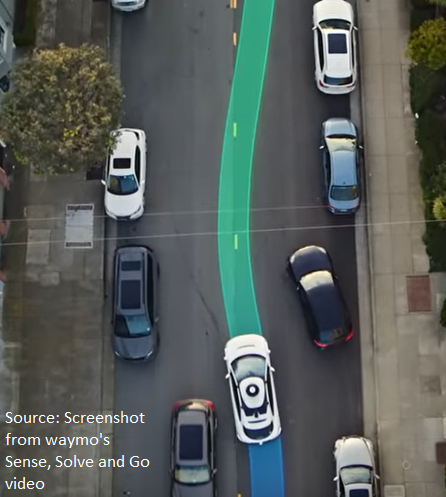
\includegraphics[scale=1]{1/waymo.png}
\caption{Waymo's L3 Data-Driven Agent}
\label{fig:waymo}
\end{center}
\end{figure}

\begin{figure}[h]
\begin{center}
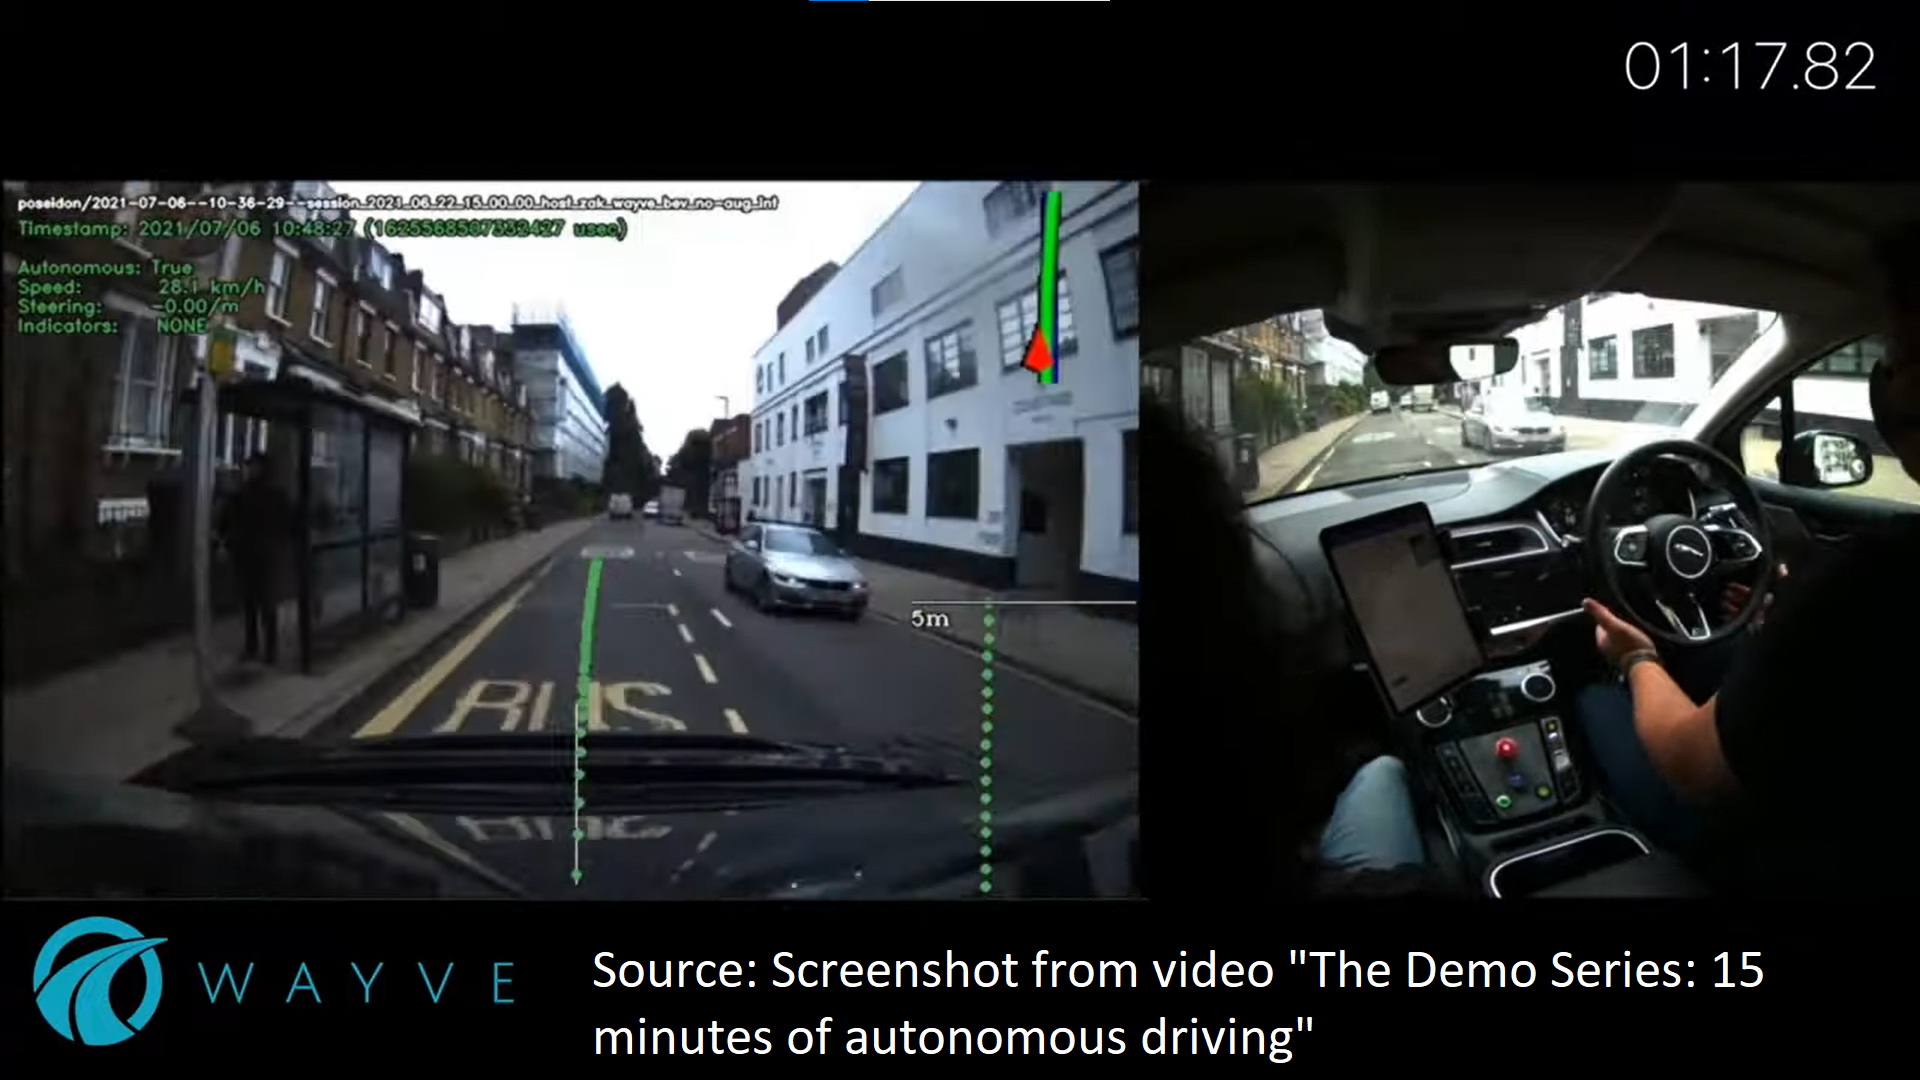
\includegraphics[scale=0.3]{1/wayve.png}
\caption{Wayve's L3 Data-Driven Agent}
\label{fig:wayve}
\end{center}
\end{figure}

\begin{figure}[h]
\begin{center}
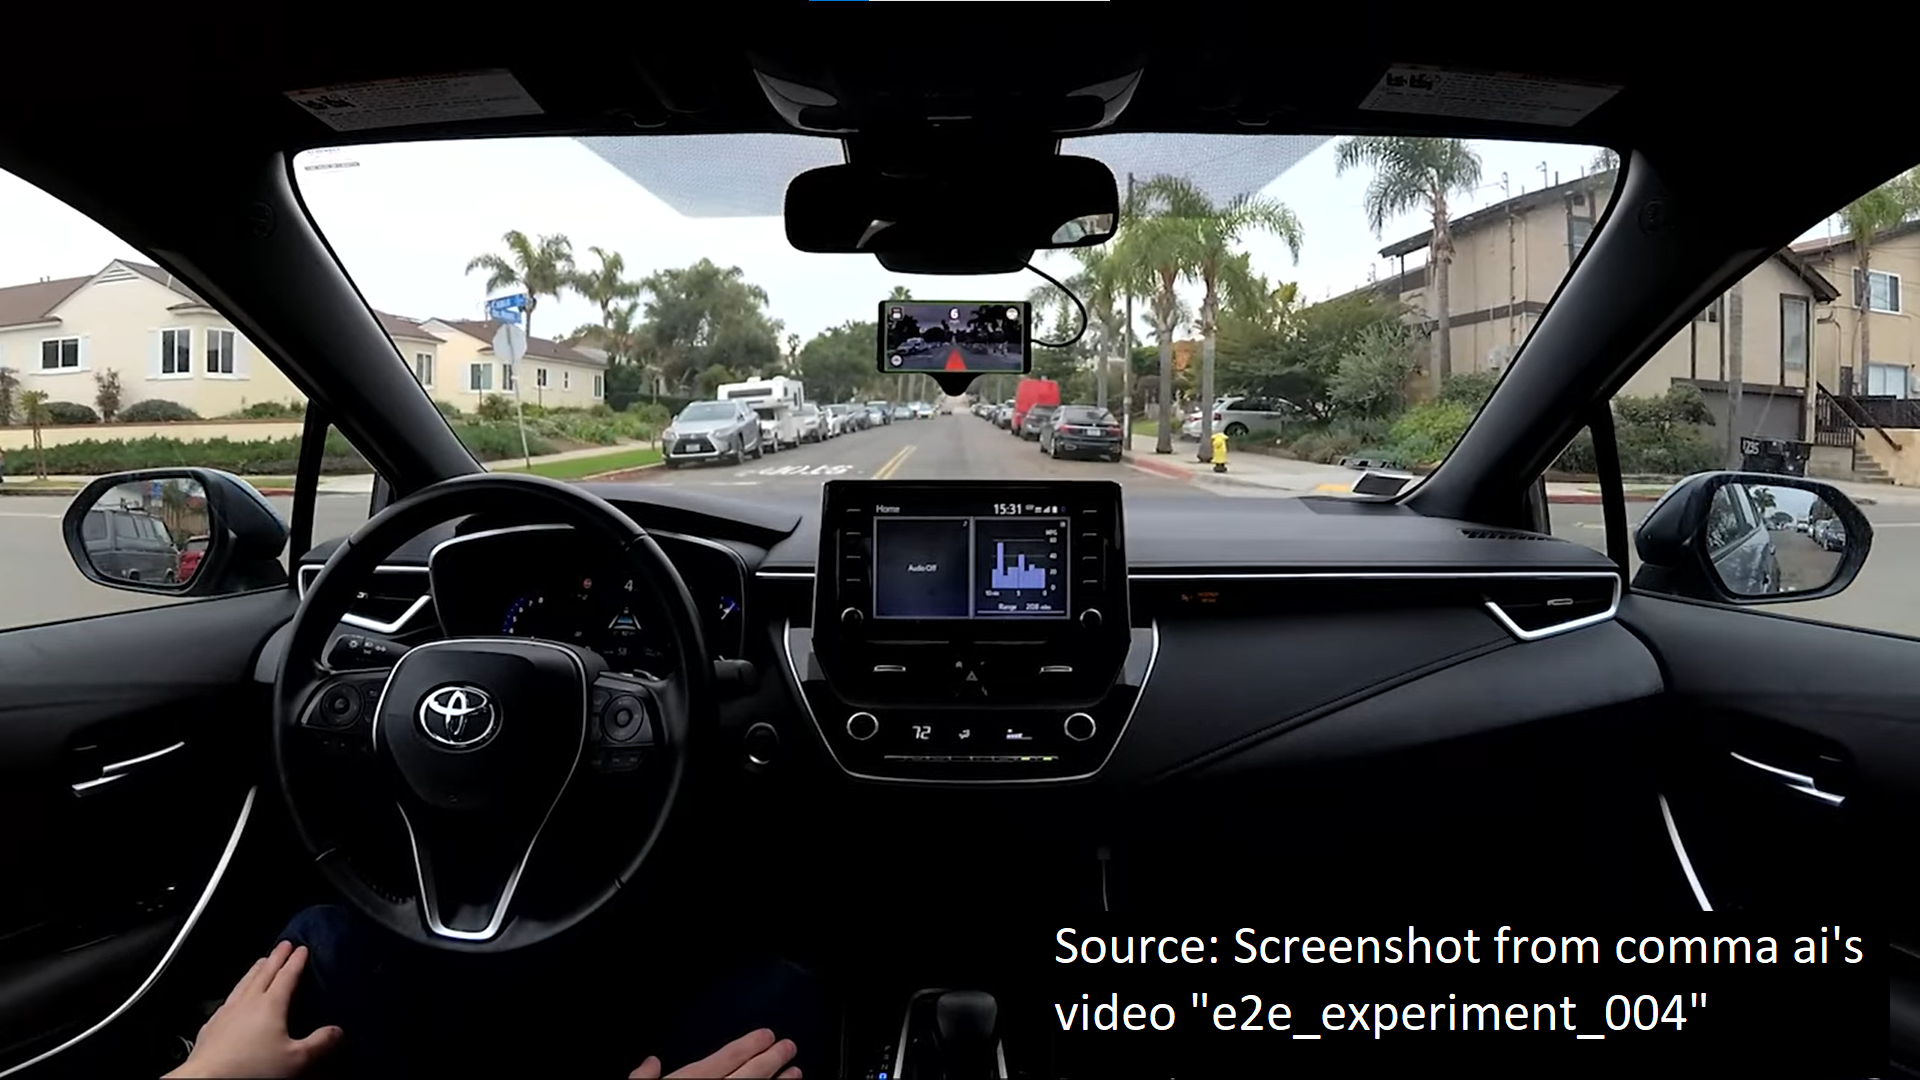
\includegraphics[scale=0.3]{1/comma.png}
\caption{Comma's L2 Data-Driven Agent}
\label{fig:comma}
\end{center}
\end{figure}

\begin{spacing}{1.5} 
\begin{sloppypar}
Research on Artificial Intelligence algorithms has rapidly progressed along with Big Data and advanced computational capabilities. AI-guided autonomous systems don't require any system-level knowledge and have great potential to optimize nonlinear systems in complex and dynamic environment. 
\end{sloppypar}
 \end{spacing}

 \begin{spacing}{1.5} 
 \begin{sloppypar}
 The Intelligent Vehicle industry is in a stand still despite of astonishing intellectual gains over the recent years. This is because SOTA Autonomous Driving technology only works reliably by overfitting on the distribution of data. The SOTA AD systems that are expert driver in ideal environment breakdown the minute it is introduced to out-of-distribution data. 
 \end{sloppypar}
  \end{spacing}


  \begin{spacing}{1.5} 
  \begin{sloppypar}
  The solution for dealing with out-of-distribution data is to incorporate knowledge-driven driving agents. With the recent advent of high-performing LLMs, implementation of knowledge-driven agents with zero-shot capabilities (meaning no fine-tuning or training the LLMs for specific downstream tasks) is feasible. 
  \end{sloppypar}
   \end{spacing}

\begin{spacing}{1.5} 
\begin{sloppypar}
In this work, we explore the use of AD task of planning as way to evaluate LLMs ability to use logical reasoning to make decisions that have short and long term effects. The AD task used in this work is an open-source gymnasium environment called 'HighwayEnv'.
\end{sloppypar}
 \end{spacing}
 
\begin{spacing}{1.5} 
\begin{sloppypar}
\section{TESTING}
Several companies that produce Intelligent Vehicles encountered accidents during testing or running. This has increased the demand for intelligent testing. Intelligent testing can identify cause of accidents and fix complications in Intelligent Vehicle systems \cite{chen2023milestones}.

There are 2 types of testing platforms. 1) Simulation Platforms and 2) Vehicles Platforms

\subsection{Simulation Platforms}
To model vehicle dynamics, tools such as 1) Carsim with ADAMS, 2) CARLA, 3) PreScan and 4) MATLAB or Simulink have been used by researchers for simulating car behaviour. Using simuluation platforms have the benefit of being able to create your own situations and test the model's behaviour in a collection of created situations.  

\subsection{Vehicles Platforms}
Some researchers use the simulation studies as first step for performance validation and conduct experimental for further validation. This is shown in the papers \cite{muller2005off} and  \cite{arifin2022steering}
\end{sloppypar}
 \end{spacing}

 
\begin{spacing}{1.5} 
\begin{sloppypar}
\section{PROBLEMS RELEVANT TO THE RESEARCH}
\begin{itemize}
    \item Lack of testing environment for LLMs with respect to Autonomous Driving planning task
    \item Lack of enough dynamic evaluation metrics 
\end{itemize}

\section{RESEARCH OBJECTIVES}
\begin{itemize}
    \item Providing a customizable platform for easy testing of LLMs Autonomous Driving planning capabilities in zero shot setting.
    \item Providing a Plug and Play dynamic evaluation metric
\end{itemize}
\section{OVERVIEW OF THE PROPOSED SYSTEM}
This work gives an interface for testing a LLM for the AD planning task. This work uses the autonomous driving environment "DuckieTown" to perform simple tasks using LLMs. The LLM chosen for this purpose is the "PHI-2" due to its small size and strong performance.
\end{sloppypar}
 \end{spacing}
 
 \begin{spacing}{1.5} 
\begin{sloppypar}
\section{ORGANIZATION OF THE REPORT}

This report is organized into 6 chapters, describing each part of the project with detailed illustrations and system design diagrams. \newline
\textbf{CHAPTER 2:} Literature Review reviews existing research, studies, and relevant literature related Autonomous Driving. Discusses the background, theories, and methodologies used by other researchers\newline 
\textbf{CHAPTER 3:} System Design describes the design of the project. Explains the architecture, components, algorithms, and any other technical details.\newline
\textbf{CHAPTER 4:} Implementation provides details about how the project was implemented. Discusses the tools, technologies, programming languages, and frameworks used.\newline
\textbf{CHAPTER 5:} Result and Analysis presents the results of the project. Analyzes the outcomes, compare them with expectations, and discuss any challenges faced during implementation.\newline
\textbf{CHAPTER 6:} Conclusion and Future Work summarizes the findings and draws conclusions. Discusses the significance of your work and its implications\newline
\end{sloppypar}
 \end{spacing}